\documentclass[10pt,a4paper]{article}
\usepackage[a4paper, left=3cm, right=3cm, top=3cm, bottom=3cm, headsep=10mm, footskip=12mm]{geometry}
\usepackage[T1]{fontenc}
\usepackage[ngerman, english]{babel}    % mehrsprachiger Textsatz
% babel: letzte Sprache in Optionen zeigt die Sprache des Dokumentes
% und kann durch den Befehl \selectlanguage{} geaendert werden
% Passen Sie die Optionen des babel-Paketes nach Bedarf an!
\usepackage{float}
\usepackage{graphicx}
\usepackage{url}
\usepackage{pdflscape}
\usepackage{mathtools}
\usepackage{amssymb, amsmath, amstext}
\usepackage{amsthm}
\usepackage{xcolor}
\usepackage{nameref}
\usepackage{siunitx}
\usepackage{makecell}
\usepackage{hyperref}
\usepackage{enumitem}
\usepackage[superscript,biblabel]{cite}
\usepackage{caption}
\usepackage{subcaption}
\usepackage{tabularx} 			% Tabellen erzeugen
\usepackage{multirow}			 % Zeilen in Tabellenbearbeitung
\usepackage{multicol} 			% Spalten in Tabellenbearbeitung 
\usepackage{lmodern}                        % Ersatz fuer Computer Modern-Schriften 
\usepackage{amsmath}                                           % zum besseren Aussehen am Bildschirm
\usepackage{booktabs} % für schönere Tabellen
\usepackage{sidecap}
\usepackage{rotating} % für die Landscape-Umgebung
\usepackage{afterpage}
\definecolor{Bluetitle}{HTML}{1F3864}
\definecolor{softbluetitle}{HTML}{274D7E}
\definecolor{Greyish}{HTML}{5A5A5A}
\definecolor{Redish}{HTML}{B2513C}
\renewcommand{\refname}{Reference}
\usepackage{array,multirow}
\newcommand{\specialcell}[2][c]{%
	\begin{tabular}[#1]{@{}c@{}}#2\end{tabular}}




\begin{document}
	
	\begin{titlepage}
		\begin{center}
			\begin{figure}[h!tbp]
				
\includegraphics[width=\linewidth]{HUlogo.PNG}
			\end{figure}
			\vspace*{2 cm}
			
			\textcolor{Bluetitle}{\textbf{\huge Atmung und Gärung}}\par
			
			\vspace*{2cm}
			
			\textcolor{Greyish}{\textbf{Versuchsdurchführende}}\par
			\textcolor{Greyish}{Oscar Moore (634083)}\par
			\textcolor{Greyish}{Fridolin Rehnig (625757)}\par
			\textcolor{Greyish}{Philipp Kunze (625468)}\par
			\textcolor{Greyish}{Daniel Kollenkirchen (625426)}\par
			\textcolor{Greyish}{Huyen Anh Nguyen (572309)}\par
			
			\vspace*{0.5cm}
			\textcolor{Greyish}{\textbf{Versuchsort}}\par
			\textcolor{Greyish}{Campus Nord, Haus 9}\par
			\textcolor{Greyish}{R2006}\par
			\vspace*{0.5cm}
			\textcolor{Greyish}{\textbf{Versuchsbetreuer}}\par
			\textcolor{Greyish}{Dr. rer. nat Christina Kühn}\par
			
			\vspace*{2 cm}
			
			\textcolor{Greyish}{09. Juli 2024}\par
			
			
			
			
		\end{center}
	\end{titlepage}
	
	\tableofcontents
	
	\section{Einführung}	
		Bei der Photosynthese gibt es zwei Hauptmechanismen der CO$_2$-Fixierung, welche jeweils von entweder C3- oder C4-Pflanzen genutzt werden und korrespondieren mit der unterschiedlichen Stärkesynthese, bzw. -akkumulierung.
		Zu den C3-Pflanzen zählen mehr als 90 $\%$ der höheren Pflanzen und diese fixieren CO$_2$ direkt im Calvin-Zyklus, im Mesophyll. In diesem Prozess wird CO$_2$  zuerst, durch das Enzym RuBisCO, in Ribulose-1,5-bisphosphat fixiert, wodurch Glycerat-3-Phosphat (3 C-Atome) entsteht, welches über mehrere Triosephosphate reduziert wird und als Vorläufer für Stärke dienen. Die Stärke wird tagsüber, als ein Produkt der lichtgetriebenen Photosynthese, im Mesophyll synthetisiert und gespeichert. Nachts hingegen wird Stärke, durch Hydrolyse, zu Glucose und Maltose abgebaut, welche aus den Chloroplasten in das Cytosol transportiert werden und dort in Saccharose umgewandelt werden, welches über das Phloem, nach der source-to-sink-Methode in andere Teile der Pflanze transportiert wird. Der Mechanismus der C3-Pflanzen ist bei hohen Temperaturen und niedrigen CO$_2$-Konzentrationen ineffizient, da die RuBisCO auch eine Oxygenase-Aktivität aufweist, was zur unerwünschten Photorespiration führt. \\
		Im Gegensatz dazu haben C4-Pflanzen einen alternativen Mechanismus entwickelt, der es ihnen ermöglicht, auch unter stressigen Umweltbedingungen effizient Photosynthese zu betreiben: die räumliche Trennung der Photosynthese und CO$_2$ -Fixierung. Die primäre CO$_2$-Fixierung findet im Mesophyll statt und von der PEP-Carboxylase durchgeführt, wobei das CO$_2$  in Phosphoenolpyruvat (PEP) fixiert wird und Oxalacetat (4 C-Atome) gebildet wird. Diese wird in Malat umgewandelt und in die Bündelscheidenzellen transportiert, wo es wiederum decarboxyliert wird, um CO$_2$ freizusetzen – dieses wird im Calvin-Zyklus weiterverarbeitet, unter anderem zu Stärke, welches auch in den Bündelscheidenzellen gespeichert wird. Der Abbau erfolgt wie bei C3-Pflanzen. Durch räumliche Trennung wird, bei C4-Pflanzen die Photorespiration verringert und die Effizienz der Photosynthese erhöht. Zudem hat die PEP-Carboxylase eine höhere CO$_2$ -Affinität und kann dieses deshalb auch bei geringeren Konzentrationen fixieren. \\
		\\
		Im 1. Versuch wird die unterschiedliche Stärkeakkumulation, mithilfe von Stärkefärbung, von Tabakpflanzen, C3-Pflanzen, und Maispflanze, C4-Pflanzen analysiert. Zudem werden beide Pflanzenarten auf anatomische Unterschiede in den Leitbündeln und Chloroplasten untersucht. Ziel des Experiments ist es, mithilfe der Analyse dieser Unterschiede, die physiologischen und anatomischen Besonderheiten der beiden Pflanzentypen besser zu verstehen. \\
		Die Grundlage der Stärkefärbung liegt in der molekularen Struktur: Stärke besteht aus Amylose und Amylopektin. Amylose und Amylopektin sind beide Polymere, bestehend aus Glukose-Untereinheiten, Ersteres ist verzweigt und Zweiteres linear. Hierbei steht jede Glucose-Untereinheit in der Kette steht zur nächsten in einem durch die glykosidische Bindung bestimmten Winkel. Das führt dazu, dass Amylose-Polymere eine regelmäßige helikale Struktur annehmen. Die Zugabe von Iod führt zu einer charakteristischen blau-schwarzen Färbung der Stärke, da die Iodmoleküle sich an unpolare Gruppen in den Hohlräumen der unverzweigten Amylose anlagern und die helikale Struktur des Moleküls stabilisieren. \\
		\\
		Im 2. Versuchsteil wird die physiologische Bedeutung des Saccharosetransporters NtSUT1 in Tabakpflanzen (Nicotiana tabacum) untersucht. Hierbei werden zuerst, die Glucose-, Fructose- und Saccharose-Gehalte in den Blättern der Saccharosetransporter-Antisense-Pflanzen untersucht und dann, die Stärkeverteilung in abgedunkelten Blättern von einem Tabak-Wildtyp und einer Saccharosetransporter-Antisense-Pflanze verglichen.\\
		Saccharosetransporter sind essentielle Proteine für den Langstreckentransport von Photoassimilaten, wie Saccharose, innerhalb der Pflanze. Sie spielen eine Schlüsselrolle bei der Phloembeladung und dem Transport von Nährstoffen von dem source-Gewebe zum sink-Gewebe. Um die Funktion des NtSUT1-Transporters zu untersuchen, werden transgene Tabakpflanzen verwendet. Genauer werden die Produktion von RNA-Molekülen initiiert, die komplementär zur mRNA des Zielgens sind, was die Translation des entsprechenden Proteins hemmt. In diesem Fall wird der Saccharosetransporter NtSUT1 in den transgenen Pflanzen herunterreguliert. Dadurch können sämtliche physiologische Veränderungen beobachten werden: die Pflanzen zeigen eine stark reduzierte Wachstumsrate, Veränderungen in Blättern, Wurzeln und Speicherorganen im Vergleich zu Kontrollpflanzen. Diese Veränderungen unterstreichen die wichtige Rolle des SUT1-Transporters im Kohlenhydratstoffwechsel und -transport.
	
	\section{Material und Methode}
	Die Versuche wurden nach dem Script durchgeführt.
	Für die Glukosebestimmung in den Blätter der Wildtyp und  NtSUT1-Antisense Tabak-Pflanze wurde ein $\o$ = 1.7 mm Stanze verwendet und beim Wildtyp eine Probe mit enem Gewicht von 41.5 mg und NtSUT1-Antisense 51.8mg entnommen.\\
	Für den Fit der Eichgerade wurde in Excel eine Trendlinie durch den Ursprung durchgeführt.
	
	\section{Ergebnis}
	\subsection{Stärkefärbung in den C3- und C4 Pflanzen}
	In der Maispflanze, welches eine C4-Pflanze ist, hat sich in den Blätter die Bündelscheidezellen verfärbt. Bei der C3-Pflanze-Tabakpflanze haben sich hingegen die Mesophylzellen verfärbt.
		\begin{figure}[H]
			\centering
			\begin{subfigure}[b]{0.31\textwidth}
				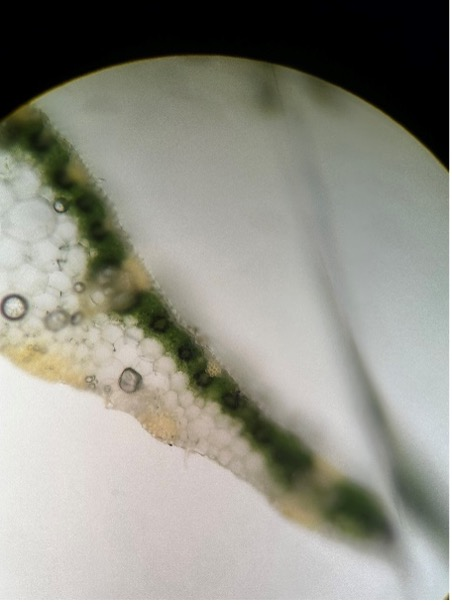
\includegraphics[width=\textwidth]{Maisquerschnitt.jpg}
				\caption{Maispflanze (C4)}
				\label{fig:mais färbung}
			\end{subfigure}
			\hfil
			\begin{subfigure}[b]{0.311\textwidth}
				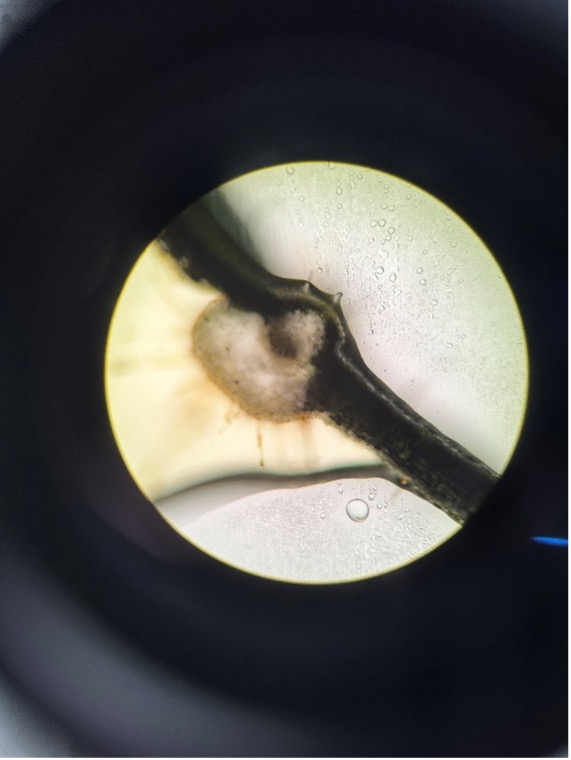
\includegraphics[width=\textwidth]{Tabakmesophyl.jpg}
				\caption{Tabakpflanze (C3)}
				\label{fig:tabakfärbung}
			\end{subfigure}

			\caption{Mikroskopische Aufnahme bei 200-Fache Vergrößerung der mit Lugol'sche Lösung gefärbten Querschnitt der Mais- und Tabakpflanze. }
			\label{fig:C3vsC4}
		\end{figure}
		
	\subsection{Wildtyp vs Antisense}
		Glukose kann photometrisch nicht direkt bestimmt werden, weswegen indirekt der Glukosegehalt durch eine gekoppelte enzymatische Reaktion bestimmt wird, wo ein anderes Substrat bei der enzymatischen Umsetzung von Glukose messbar ist.\\
		 NAD$^+$ $\longrightarrow$ NADH ist bei $\lambda$ = 340 nm photometrisch messbar.
		 Die Menge der die an NAD$^+$ umgesetzt wird, kann mit der Glukosemenge gleichgesetzt werden.
		 Das kann so angenommen werden, da die Substrate ATP und NAD$^+$ für die beiden Reaktionen in Gleichung (\ref{reaktionsgleichung}) in Überschuss eingesetzt wird.\\
		 Mittels einer Eichgerade (siehe Figurre \ref{eq: eichkurve}) kann dann ddas Glucosegehalt ermittelt werden.

		\begin{equation}\label{reaktionsgleichung}
			\begin{split}
				\text{Glukose} + \text{ATP} &\xlongrightarrow{\text{Hexokinase}} \text{Glucose-6-P + ADP}\\
				\text{Gucose-6-P +NAD$^+$} &\xlongrightarrow{\text{Gucose-6-P-Dehydrogenase}} \text{Gluconat-6-P + NADH +H$^+$}
			\end{split}
		\end{equation}
		
		Bei der Bestimmung der unbekannten Probe und der Extrakte, wurde die Extinktion (jeweils Doppelwerte) vor Zugabe der Hexokinase und 15 minuten nach der Zugabe bestimmt und nach Gleichung (\ref{eq:delta E}) $\Delta E$ berechnet. Die Glukosemenge lies sich dann durch die Steigung der Eichgeraden und den berechneten Extinktionswerten nach Gleichung (\ref{eq: eichkurve}) errechnen. Photometrisch wurde eine Glukosegehalt von 19$\mu g$ (5.3 mM) für die unbekannte Probe gemessen. Das NtSUT1-Antisense Extrakt enthielt ca. 1.23$\frac{\mu g}{\text{mg Frischgewicht}}$ Glukose und das Wildtyp Extract ca. 2.05$\frac{\mu g}{\text{mg Frischgewicht}}$ (sieht Table \ref{tab:Glucosegehalt in Tabak}) .\\
		Die Rechnung kann im Abschnitt \ref{rechenweg} nachvollzogen werden.
		
		\begin{equation}\label{eq:delta E}
			\overline{E}_{nachher} - \overline{E}_{vorher}=\Delta E
		\end{equation}
		\begin{equation}\label{eq: eichkurve}
			\Delta E = a \cdot m \leftrightarrow m=\frac{\Delta E}{a}
		\end{equation}
		\begin{figure}[H]
			\centering
			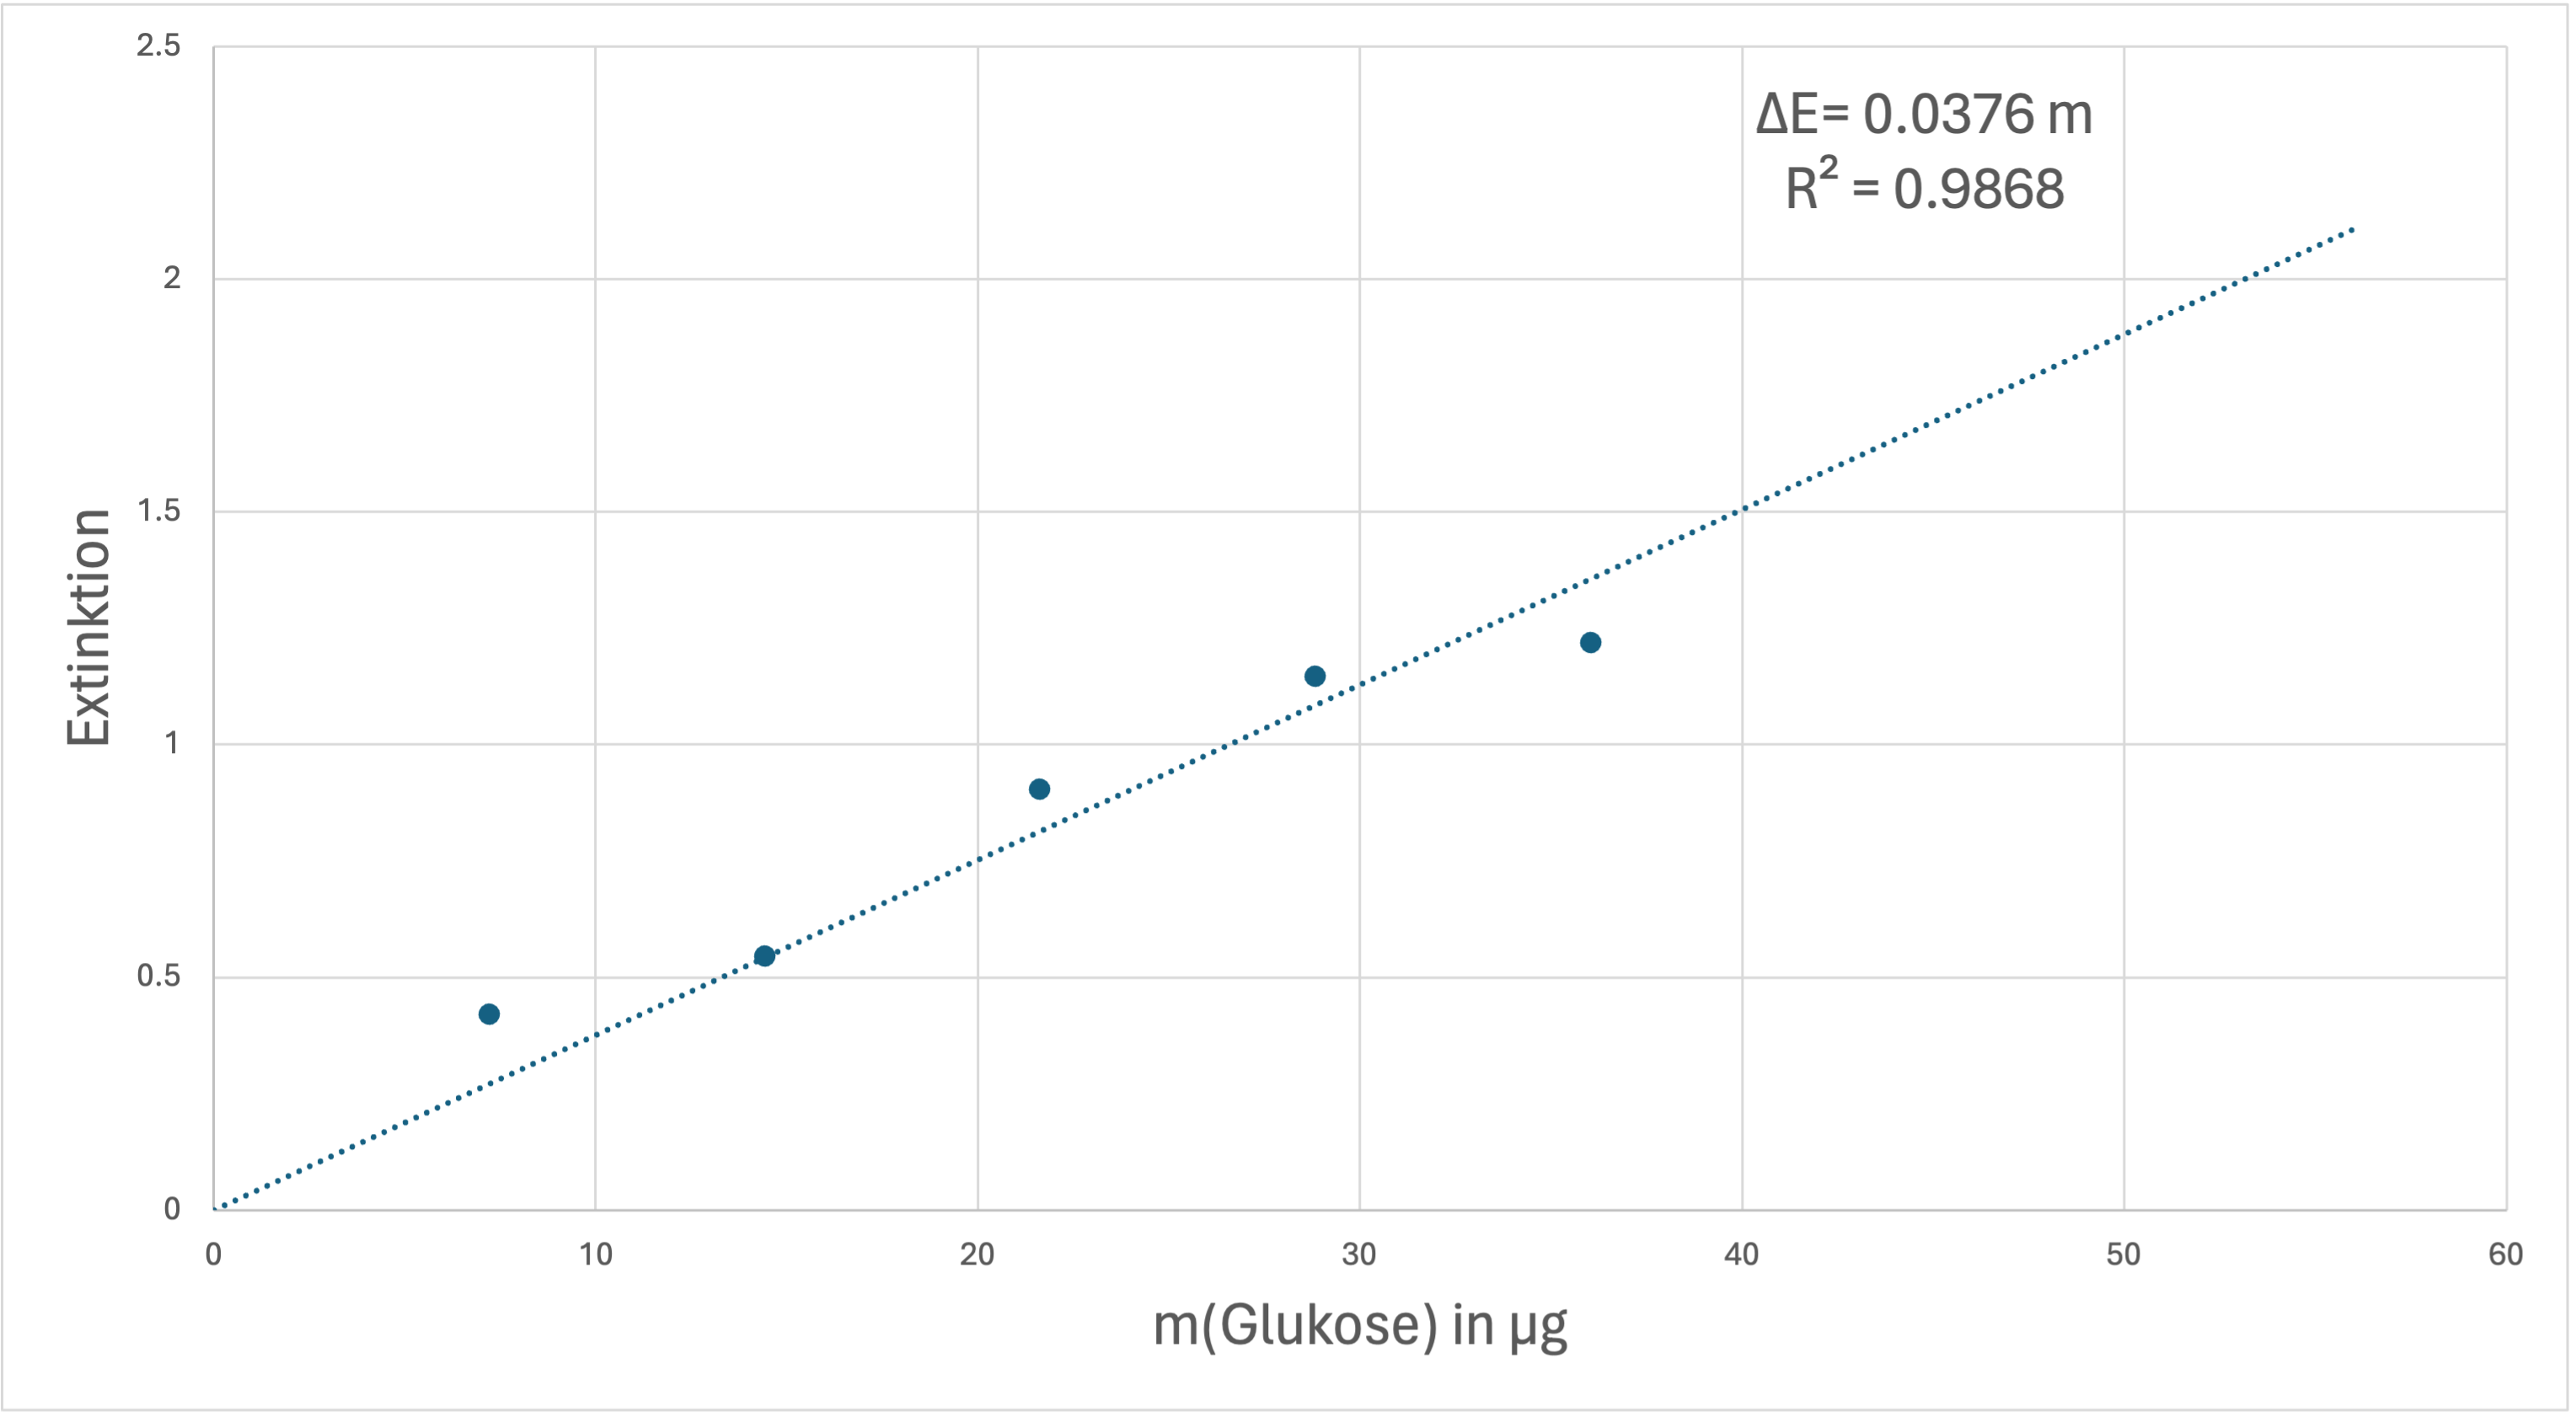
\includegraphics[width=0.75\linewidth]{Eichgerade.png}
			\caption{Eichgerade von Glukose. Die Abhängigkeit der Extinktion bzw optische Dichte von der Masse von Glucose bei  $\lambda$ = 340nm.}
			\label{Abbildung 1}
		\end{figure}
		
		\begin{table}[H]
			\centering
			\begin{tabular}{ccc}
				\toprule
				& Glukosemenge in $\mu$g & Glukosemenge in $\mu$g \\
				&& pro mg Frischgewicht \\ 
				\midrule
				WT & 4.43 & 1.23\\
				Antisense & 7.38 & 2.05\\
				Unbekannt & 19.03 & -\\
				\bottomrule
			\end{tabular}
			\caption{Glukosegehalt in den Blattextraktes vom Wildtype und NtSUT1-Antisense der Nicotiana tabacum Pflanze und der Glukosegehalt von der unbekannte Probe.}
			\label{tab:Glucosegehalt in Tabak}
		\end{table}
		
		\subsubsection{Stärkefärbung der abgedunkelte Blätter}
		Nach dem die abgedunkelten Blätter beider Pflanzen (Tabak Wildtyp, Tabak Antisense) durch die Lugol‘sche Lösung gefärbt wurden konnte man schon nach kurzer Zeit eine deutliche Färbung sowohl des Antisense-Tabakblattes als auch des Wildtyps erkennen. Der Wildtyp zeigte eine komplett schwarze Färbung des gesamten Blattes (siehe Figure \ref{fig:wildtyp färbung} ). Die Antisense-Pflanze zeigte ebenfalls eine schwarze Färbung, jedoch waren die Blattadern, sowie ein kleiner Bereich um die Blattadern nicht gefärbt (siehe Figure \ref{fig:antisense fail färbung} ). Interessant war vor allem, dass die Färbung des Wildtyp-Blattes anderer Gruppen ganz anders aussah. Wie in Figure \ref{fig:antisensefärbung} zu erkennen ist, hat sich das Blatt hier überhaupt nicht schwarz verfärbt. 
		
				
		\begin{figure}[H]
			\centering
			\begin{subfigure}[b]{0.3\textwidth}
				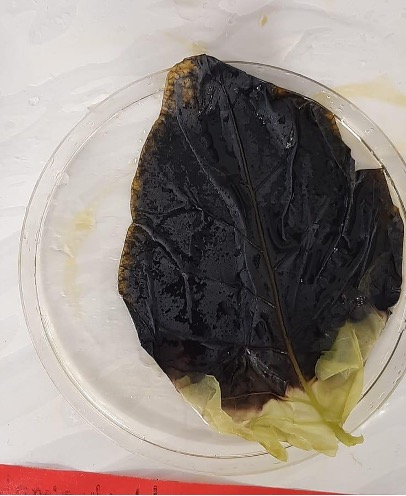
\includegraphics[width=\textwidth]{wildtypblatt.jpg}
				\caption{Wildtyp}
				\label{fig:wildtyp färbung}
			\end{subfigure}
			\hfill
			\begin{subfigure}[b]{0.345\textwidth}
				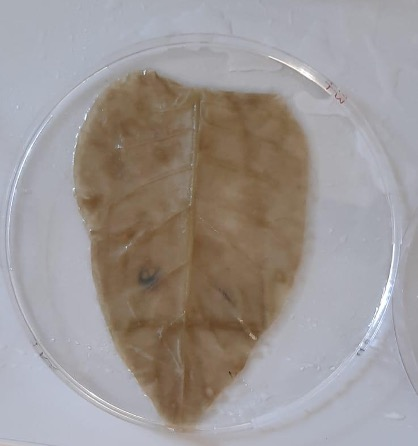
\includegraphics[width=\textwidth]{antisenseblatt.jpg}
				\caption{Antisense}
				\label{fig:antisensefärbung}
			\end{subfigure}
			\hfill
			\begin{subfigure}[b]{0.26\textwidth}
				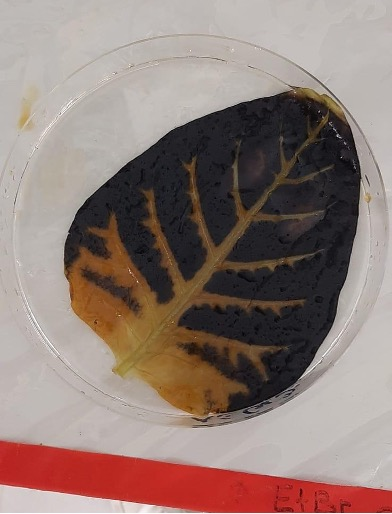
\includegraphics[width=\textwidth]{antisenseblattfail.jpg}
				\caption{Antisense von einer anderen Gruppe}
				\label{fig:antisense fail färbung}
			\end{subfigure}
			\hfill
			\caption{Die mit Alufolie abgedeckte Blätter der Nicotiana tabacum Pflanze der Wildtyp und NtSUT1-Antisense-Typ wurde mit 80$\%$ Ethanollösung für 30 min bei 70°C entfärbt und dann mit Lugol'sche Lösung gefärbt. }
			\label{fig:dunkelfärbung}
		\end{figure}
		
	
	\section{Diskussion}
	\subsection{Stärkeverteilung in den C3- und C4-Pflanzen}
	Wie die Ergebnisse anschaulich verdeutlichen, wird Stärke in C3-Pflanzen (siehe Figure \ref{fig:tabakfärbung}) und C4-Pflanzen (siehe Figure \ref{fig:mais färbung}) in unterschiedlichen Zelltypen gespeichert. In C3-Pflanzen wird die Stärke in den Mesophyllzellen, in C4-Pflanzen in den, die Leitbündel umgebenden, Bündelscheidenzellen gespeichert. Dies lässt sich durch den, von den C4-Pflanzen abgewandelten Photosynthese Weg, erklären. \\
	In den Mesophyllzellen der C4-Pflanzen wird CO$_2$ zunächst durch die Pep-Carboxylase in die vier Kohlenstoffhaltigen Verbindungen Malat/Aspartat umgewandelt. Dies wird anschließend in die Bündelscheidenzellen transportiert, dort zu CO$_2$ Decarboxyliert, welches anschließend in den Calvin-Zyklus eingespeist wird und durch die Rubisco fixiert wird. Die synthetisierte Stärke wird anschließend auch in den Bündelscheidenzellen gespeichert.
	In C3 Pflanzen findet die Carboxylierung durch die Pep-Carboxylase nicht statt. Stattdessen wird CO$_2$ ohne Umwandlung direkt in den Mesophyllzellen in den Calvin-Zyklus eingespeist und dort von der Rubisco fixiert. Die Speicherung von Stärke findet daher logischerweise auch in den Mesophyllzellen statt.\\
	Aus diesen Unterschieden ergibt sich ein Vorteil für C3-Pflanzen bei gemäßigten Temperaturen. Ein Nachteil jedoch bei niedrigen CO$_2$ Konzentrationen da dann die Photorespiration steigt und die Rubisco statt CO$_2$ Sauerstoff bindet und so ein Energieverlust eintritt. Auch haben C3-Pflanzen gegenüber den C4-Pflanzen einen Nachteil, wenn die Temperatur hoch ist, da sie ihre Stomata länger und vorallem bei Tag öffnen müssen, um Gasaustausch betreiben zu können und die Rubisco bei höheren Temperaturen affiner gegenüber Sauerstoff wird. C4-Pflanzen profitieren vom jeweils gegenteiligen, haben aber durch ihren komplizierteren Stoffwechselweg einen höheren Energie bedarf, der sich bei gemäßigten Temperaturen nicht auszahlt.\\
	Durch diese Unterschiede der Photosynthese Mechanismus betreffend, sind auch anatomische Unterschiede zu erklären. Da bei C4-Pflanzen Malat in die Bündelscheidenzellen transportiert wird, sind die Mesophyllzellen kreisrund (Kranzanatomie) um diese angeordnet und bilden nicht ausschließlich ein weit entferntes Palisadenparenchym wie in den C3-Pflanzen. Des weiteren verfügen die Bündelscheidenzellen der C4-Pflanzen auch über Chloroplasten. 
	
	
	\subsection{Wildtyp vs Antisense}
	\subsubsection{Glukosegehalt in den Blätter}
	Der deutliche Unterschied im Zuckergehalt der Wildtyp und Antisense Pflanzen entspricht unseren Erwartungen. Durch die Antisense Inhibierung des Saccharosetransporters SUT1, wird die Weiterleitung der Photoassimilate an das Phloem, für den Langstreckentransport verhindert. Es kommt somit in den Blättern der Transgenen Pflanzen zu einer Akkumulation an Saccharose und demnach auch zu einer höheren gemessenen Glukosekonzentration, als in den Wildtyp Pflanzen, welche das Phloem problemlos mit Saccharose beladen können. \\
	Dadurch dass jeweils nur Doppelwerte gemessen wurde, können die Werte, wie die c(unbekannte Glucoseprobe) = 5.3 mM vom wahren Wert abweichen, da R$^2$ = 0.9868 beträgt.
	Mit mehr Mehrfachmessungen kann der Fehler minimiert werden.
	\subsubsection{Stärkefärbung von abgedunkelten Blätter}
	Mittels der Lugol’schen Lösung konnte die Stärkeverteilung in den Blättern sichtbar gemacht werden. Dabei lagerten sich die Polyiodid-Ketten aus der Lugol’schen Lösung in die helikale Struktur der Stärke ein. Dabei interagieren sie mit den Hydroxy-Gruppen der Kohlenhydrate. Dies wurde als violett bis schwarze Färbung sichtbar\cite{unterrichtsmaterial}. Daraus lässt sich ableiten, dass in den Blättern des Wildtyps Stärke vorhanden war. Es war keine Variation der Färbung in unterschiedlichen Geweben sichtbar. In den Blättern der Antisense-Pflanze befand sich keine Stärke in den Blattadern, jedoch in allen anderen Geweben.\\
	Bei der Lichtreaktion der Fotosynthese werden in den Blättern große Mengen an Assimilationsstärke gebildet. Stärke ist eine Speicherform von Kohlenhydraten, die während der Lichtreaktion der Photosynthese gebildet wurden. Sie besteht aus zwei Glucose-Polymeren, Amylopektin und Amylose. Die Stärke kann zum späteren Zeitpunkt wieder in nutzbare Zucker umgewandelt werden. Das geschieht beispielsweise in der Nacht, wenn keine Lichtreaktion möglich ist. Im Dunkeln wird die Stärke zu Glukose und Maltose abgebaut, wobei Maltose im Cytoplasma in Saccharose umgewandelt wird, und anschließend über den Phloemtransport in der Pflanze verteilt werden kann \cite{Kadereit} . In diesem Versuch wurden die untersuchten Blätter über mehrere Tage keinem Licht ausgesetzt, weshalb in den Blättern keine Lichtreaktion der Photosynthese mehr betrieben werden konnte. Dadurch konnte auch keine neue Stärke gebildet werden. Um also weiterhin die Pflanze mit nötigen Kohlenhydraten zu versorgen, wurden die aufgebauten Stärkereserven genutzt und in den Transportzucker Saccharose umgewandelt, um über das Phloem exportiert zu werden. Deshalb ist zu erwarten, dass nach längerer Zeit ohne Licht, keine oder wenig Stärke in den Blättern nachzuweisen ist. Dies konnte zumindest beim Blatt des Wildtyps in unserem Versuch nicht nachgewiesen werden. Jedoch ist anzunehmen, dass der Versuch fehlerhaft durchgeführt wurde, denn bei anderen Gruppen konnte sehr wohl eine Entfärbung des Wildtyp Blattes festgestellt werden (siehe Figure \ref{fig:wildtyp färbung} ). Mehr zu den möglichen Fehlerquellen später. Es sollte also beim Wildtyp keine Färbung durch die Lugol’sche Lösung möglich sein. Im Vergleich dazu zeigte die Antisense-Pflanze eine Färbung des Blattes, ausgenommen den Blattadern. Da es sich, wie oben bereits erläutert, um eine Pflanze mit inhibiertem Saccharosetransporter handelte, konnte in der transgenen Pflanze der Saccharosetransport aus den Zellen nur eingeschränkt stattfinden. Durch diese Einschränkung wurde in den Zellen auch wenig Saccharose gebildet, da es sich sonst in den Zellen angestaut hätte. Auch bei Dunkelheit, musste die gespeicherte Stärke nicht abgebaut werden, da kein Bedarf an Saccharose vorhanden war. Die hellen Bereiche der Blattadern lässt sich damit erklären, dass hier hauptsächlich Leitgewebe sitzt. Da es sich bei der Inhibierung nur um ein Knock-Down und kein vollständiges Knock-Out handelte, konnten die Zellen in geringem Umfang weiterhin Saccharose exportieren. Das wurde vorrangig in der nahen Umgebung des Leitgewebes sichtbar, da sich hier weniger Stärke nachweisen ließ.\\
	Die Ergebnisse des Versuchs waren teilweise nicht wie erwartet. Die erwartete Entfärbung des Wildtyp Blattes konnte bei uns nicht festgestellt, jedoch von anderen Gruppen bestätigt werden. Die mögliche Ursache für diesen Fehler war, dass das Blatt nicht vollständig oder nicht lange genug abgedunkelt war, wodurch entweder weiterhin eine Lichtreaktion stattfinden und damit Stärke gebildet werden konnte oder noch zu viel Stärke im Blatt gespeichert war. Dies ist die naheliegendste Fehlerquelle, andere Fehler können jedoch nicht ausgeschlossen werden.
	

	\section{Anhang}
		\subsection{Rohdaten}
		
		\begin{table}[H]
			\centering
			\begin{tabular}{ccccc}
				\toprule
				Probe & \multicolumn{2}{c}{E$_{vorher}$} & \multicolumn{2}{c}{E$_{nachher}$} \\
				\midrule
				7.2 $\mu$g Glukose& - & - & 0.427 & 0.418\\
				14.4 $\mu$g Glukose& - & - & 0.536 & 0.556\\
				21.6 $\mu$g Glukose& - & - &0.88 & 0.930\\
				28.8 $\mu$g Glukose&-&-&1.062 & \textcolor{Redish}{1.233}\\
				36.03 $\mu$g Glukose&-&-&1.237&\textcolor{Redish}{1.201}\\
				\midrule
				Unbekannte & - &- &0.781 & 0.65\\
				Wildtyp & 0.391 & 0.375 & 0.502 & 0.597\\
				Antisense & 0.368 & 0.331 & 0.516 & 0.738\\
				\bottomrule
			\end{tabular}
			\caption{Photometrische Daten vor der Hexokinasen Zugabe und 15 Minuten nach der Zugabe.}
			\label{tab:Extinktion}
		\end{table}
		
	
	\subsubsection{Rechenweg für die Bestimmung des Glukosegehalt}\label{rechenweg}
	Ein Beispielrechnung wie das Ergebnis des Wildtypes in Table \ref{tab:Glucosegehalt in Tabak} bestimmt wurde.\\
	Zuerst wird $\Delta$ E nach Gleichung \ref{eq:delta E} bestimmt.\\
	
	\begin{equation}\nonumber
		\Delta E = \frac{0.502 + 0.597}{2} -  \frac{0.391 + 0.375}{2} = 0.167
	\end{equation}
	Dann wird die Masse von Glukose in der 20 $\mu$L  Probevolumen mit der Gleichung \ref{eq: eichkurve} bestimmt.\\
	Das Parameter a ist hier die Steigung und beträgt 0.0376 $\mu$g$^{-1}$.\\
	\begin{equation}\nonumber
		m = \frac{\Delta E}{a} = \frac{0.167}{0.037} = 4.43 \mu g
	\end{equation}
	Da die Masse von der Glucose nur in den 20$\mu$L bestimmt wurde, musst diese noch auf die 500 $\mu$L  Probevolumen des Wildtypextraktes hochgerechnet werden.\\
	
	\begin{equation}\nonumber
		\begin{split}
			4.43 \mu g &\equiv 20 \mu L\\
			m_{ges} &\equiv 500 \mu L \rightarrow Dreisatz\\
		\\
			m_{ges} & = \frac{4.43 \mu g  \cdot 500 \mu L}{20 \mu L} = 110.7 \mu g
		\end{split}
	\end{equation}
	Mit der Gesamtmasse m$_{ges}$ kann dann pro mg Frischegewicht runtergerechnet werden.\\
	\begin{equation}\nonumber
		\frac{110.7 \mu g}{41.5 mg} = 1.23 \frac{\mu g}{mg}
	\end{equation}

	
	


	\addcontentsline{toc}{section}{References}
	\bibliographystyle{plainurl}
	\nocite{*}
	\bibliography{Literatur}
	\newpage

	
\end{document}